\documentclass[11pt]{beamer}
\usetheme{Warsaw}
\usepackage[utf8]{inputenc}
\usepackage[spanish]{babel}
\usepackage{amsmath}
\usepackage{amsfonts}
\usepackage{amssymb}
\usepackage{graphicx}
\author{N.Pérez-Medina}
\title{Capítulo 2 - Herramientas lineales y consideraciones generales}
\setbeamercovered{transparent} 
\setbeamertemplate{navigation symbols}{} 
\logo{
\includegraphics[scale=0.04]{logo_fing_uach_bn.png} } 
\institute{\textbf{FING - UACH}
	\\
	\begin{small}
	\textit{Análisis de series de tiempo no lineales}\\
	\textbf{Catedrático:} Dr. José Luis Herrera Aguilar
	\end{small}		
	} 
\date{\today} 
\subject{Series de tiempo} 


% Para tener un morado coqueto
\definecolor{lightPurple}{RGB}{186, 146, 209} % Morado claro
\definecolor{darkPurple}{RGB}{98, 54, 150}    % Morado oscuro
\setbeamercolor{structure}{fg=darkPurple} % Color principal para estructuras
\setbeamercolor{frametitle}{bg=darkPurple, fg=white} % Título del marco
\setbeamercolor{block title}{bg=darkPurple, fg=white} % Título de bloques
\setbeamercolor{block body}{bg=lightPurple!30, fg=black} % Cuerpo de bloques

\begin{document}

\begin{frame}
	\maketitle
\end{frame}

\begin{frame}
	\tableofcontents
\end{frame}

\section{Estacionariedad y muestreo}
\begin{frame} 
\tableofcontents[currentsection] % Solo muestra la sección actual
\end{frame}

\begin{frame}{Sobre la reproducibilidad}
	\begin{block}{En general}
		Una medición científica de cualuqier tipo es en principio más \textit{útil} cuanto más \textit{reproductible} sea.
	\end{block}
	\begin{block}{¿Cómo se relaciona?}
		\begin{itemize}
			\item Una serie temporal es una forma de medición científica.
			\item La reproducibilidad está estrechamente vinculada a la estacionariedad.
		\end{itemize}
		
	\end{block}
\end{frame}

\begin{frame}{Estacionareidad débil.}
	\begin{block}{Condiciones}
		\begin{itemize}
			\item Media constante
			\item Varianza constante
		\end{itemize}
	\end{block}
	\centering
	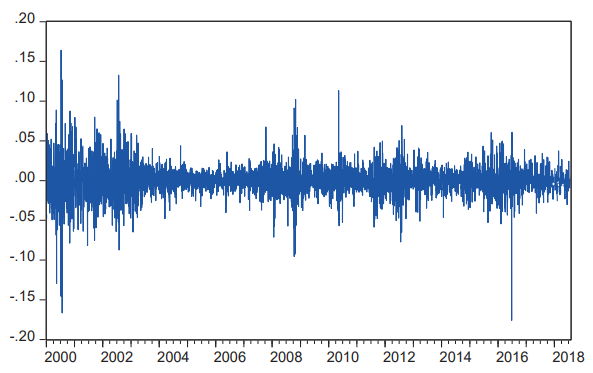
\includegraphics[scale=0.5]{idea-grafica.png} 
\end{frame}

\begin{frame}{De manera (un poco) más formal}
	\begin{block}{Para denominar una señal estacionaria:}
		Los fenómenos que afectan a los datos deben ser regulares y repetirse con suficiente frecuencia dentro de cada ventana de tiempo.
	\end{block}
	
	\begin{block}{La propiedad clave}
		 Dentro de cualquier ventana de tiempo de un tamaño $s$, la distribución de los datos debe ser la misma.
	\end{block}
\end{frame}

\section{Pruebas de estacionareidad}
\begin{frame} 
\tableofcontents[currentsection] % Solo muestra la sección actual
\end{frame}

\begin{frame}{Primer requisito}
	\begin{block}{}
		La serie temporal debe cubrir un intervalo de tiempo mucho mayor que la escala de tiempo caraceterística más larga que sea relevante para la evución del sistema
	\end{block}
	
	\begin{block}{Ejemplo}
		La concentración de azúcar en la sangre de un ser humano está impulsada por el consumo de alimentos y, por tanto, sigue aproximadamente un ciclo de 24 horas. 
		
		Si esta cantidad se registra durante 24 horas o menos, el proceso debe considerarse no estacionario, sin importar cuántos puntos de datos se hayan
tomado durante ese tiempo.
	\end{block}
\end{frame}

\begin{frame}{Primer requisito}
	\begin{block}{}
		La escala de tiempo relevante más larga puede estimarse como el inverso de la frecuencia más baja que aún contiene una fracción significativa de la potencia total de la señal. 
	\end{block}
	\begin{block}{}
		Una serie temporal solo puede considerarse estacionaria en escalas de tiempo mucho mayores.
	
	\end{block}
\end{frame}

\section{Correlaciones lineales y el espectro de potencia.}
\begin{frame} 
\tableofcontents[currentsection] % Solo muestra la sección actual
\end{frame}

\begin{frame}{Entradas irregulares}
	\centering
	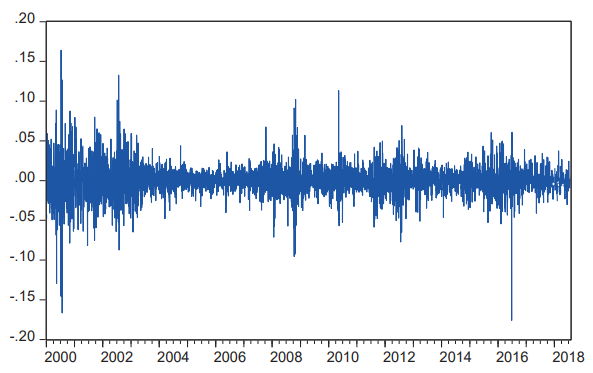
\includegraphics[scale=0.5]{idea-grafica.png} 
\end{frame}

\begin{frame}{Entradas irregulares}
	\begin{block}{}
		Entonces, cada valor $s_n$ puede interpretarse como una muestra de una distribución de probabilidad $P(s)$ \textit{subyacente} al proceso estocástico de entrada.
	\end{block}
	
	\begin{block}{}
		Un proceso estocástico se denomina \textit{estacionario} si estas probabilidades son constantes en el tiempo $P(s_n) = P(s)$
	\end{block}
	
	\begin{block}{}
		Como únicamente disponemos de la serie temporal de salidas y no de la entrada, podemos inferir características de $P(s)$ a partir de los datos observados.
	\end{block}
\end{frame}

\begin{frame}{Estimaciones}	
\begin{block}{Media}
	La \textit{media} de la \textbf{distribución de probabilidad} $p(s)$, definida como:
	\begin{equation}
		\langle s \rangle := \int_{-\infty}^{\infty} ds' \, s' \, p(s'), 
	\end{equation}

	puede estimarse mediante la \textit{media} de la \textbf{serie temporal finita}

	\begin{equation}
		\langle \hat{s} \rangle_N = \frac{1}{N} \sum_{n=1}^N s_n ,
	\end{equation}

	donde $\langle \cdot \rangle_n$ denota el promedio en el tiempo y $N$ es el número total de mediciones en la serie temporal. 
\end{block}

\end{frame}

\begin{frame}{Estimaciones}
\begin{block}{Varianza}
	La \emph{varianza} de la \textbf{distribución de probabilidad} se estimará mediante la \textit{varianza} de la \textbf{serie temporal finita}:

	\begin{equation}
		\sigma^2 := \langle (s - \langle s \rangle)^2 \rangle = \int_{-\infty}^{\infty} ds' \, (s' - \langle s \rangle)^2 p(s'),
	\end{equation}

	\begin{equation}
		\hat{\sigma}^2 = \frac{1}{N-1} \sum_{n=1}^N (s_n - \langle \hat{s} \rangle_N)^2 
= \frac{1}{N-1} \left( \sum_{n=1}^N s_n^2 - N (\langle \hat{s} \rangle_N)^2 \right)
	\end{equation}

	Nos referiremos a $\sigma$ como la desviación estándar o la amplitud rms (\emph{root mean squared}), en contraste con la \emph{varianza} $\sigma^2$.
\end{block}

\end{frame}

\begin{frame}{Estimaciones}
	\begin{block}{Sin embargo}
		Para estas dos cantidades, el\textit{ orden temporal de las mediciones} es irrelevante y, por lo tanto, no pueden aportar información sobre la evolución temporal de un sistema.
	\end{block}
	
	\begin{block}{}
		Dicha información puede obtenerse a partir de las \emph{autocorrelaciones} de una señal.
	\end{block}
\end{frame}

\begin{frame}{Estimaciones}
	\begin{block}{Autocorrelaciones}
	La autocorrelación con retardo $\tau$ está dada por

\begin{equation}
c_{\tau} = \frac{1}{\sigma^2} \langle (s_n - \langle s \rangle)(s_{n-\tau} - \langle s \rangle) \rangle 
= \frac{\langle s_n s_{n-\tau} \rangle - \langle s \rangle^2}{\sigma^2}
\end{equation}

La estimación de las autocorrelaciones a partir de una serie temporal es sencilla siempre que el retardo $\tau$ sea pequeño en comparación con la longitud total de la serie. Por lo tanto, las estimaciones $\hat{c}_\tau$ son razonables únicamente para $\tau \ll N$.  
	\end{block}
\end{frame}

\begin{frame}{Sobre las autocorrelaciones}
	\begin{block}{Autocorrelaciones y procesos estocásticos}
		Los procesos estocásticos tienen autocorrelaciones decrecientes, pero la tasa de decaimiento depende de las propiedades del proceso.
	\end{block}
	
	\begin{block}{Autocorrelaciones y sistemas caóticos deterministas}
		Las autocorrelaciones de señales provenientes de sistemas caóticos deterministas típicamente decaen de forma exponencial con el incremento del retardo.
	\end{block}
\end{frame}

\begin{frame}{Nuestro amigo Fourier}
	\begin{block}{Características}
		La \emph{transformada de Fourier} establece una correspondencia uno a uno entre la señal en ciertos instantes de tiempo (\emph{dominio temporal}) y cómo ciertas frecuencias contribuyen a la señal, así como la forma en que las fases de las oscilaciones se relacionan con las fases de otras oscilaciones (\emph{dominio frecuencial}).
	\end{block}
	\[
        \underbrace{\text{Señal en el tiempo } x(t)}_{\text{dominio temporal}}
        \quad \overset{\text{Fourier}}{\longleftrightarrow} \quad
        \underbrace{\text{Contribución de cada frecuencia } X(f)}_{\text{dominio frecuencial}}
        \]
\end{frame}

\begin{frame}{Nuestro amigo Fourier}
	\begin{block}{Transformada de Fourier}
		Aparte de diferentes convenciones respecto a la normalización, la transformada de Fourier de una función $s(t)$ está dada por

\begin{equation}
\tilde{s}(f) := \frac{1}{\sqrt{2\pi}} \int_{-\infty}^{\infty} s(t) e^{2\pi i f t} dt
\end{equation}

y la de una serie temporal discreta y finita por

\begin{equation}
\tilde{s}_k = \frac{1}{\sqrt{N}} \sum_{n=1}^N s_n e^{2\pi i k n / N}
\end{equation}

Aquí, las frecuencias en unidades físicas son $f_k = k / (N \Delta t)$, donde $k = -N/2, \ldots, N/2$ y $\Delta t$ es el intervalo de muestreo.
	\end{block}
\end{frame}

\begin{frame}{Espectro de potencia}
	\begin{block}{Espectro de potencia y Transformada de Fourier}
		El \emph{espectro de potencia} de un proceso se define como el módulo al cuadrado de la transformada de Fourier continua, $S(f) = |\tilde{s}(f)|^2$. 
	\end{block}
\end{frame}

\begin{frame}{Espectro de potencia y función de autocorrelación}
	\begin{block}{\textit{Teorema de Wiener-Kinchin}}
		Establece que la transformada de Fourier de la función de autocorrelación es igual es espectro de potencia.
	\end{block}
	\begin{block}{\textit{Teorema de Parseval}}
		La potencia total crece linealmente con la longitud de la serie temporal y puede calcularse tanto en el dominio temporal como en el frecuencial
\begin{equation}
S = \sum_{n=1}^N |s_n|^2 = \sum_{k=-N/2}^{N/2} |\tilde{s}_k|^2 
\end{equation}
	\end{block}
\end{frame}
\section{Ejercicios}
\begin{frame}{Pasamos a los ejercicios}
	\begin{center}
		\Huge
		Gracias
	\end{center}
\end{frame}
\end{document}

